\subsubsection{Advection stabilization benchmarks}

The underlying PDEs of the temperature and compositional field are typically advection-dominated and as such, require a stabilization scheme, see \ref{sec:advection-stabilization} for
an introduction for the methods implemented in \aspect{}.

We have several benchmarks to test the robustness, quality of solutions (size of overshoots, smearing of sharp interfaces). Here, we give a short summary of the benchmarks implemented:
\begin{itemize}
 \item Dropping box (\texttt{benchmarks/drop\_*.prm}): This is a simple 2d box with a prescribed, constant, vertical velocity. An initial condition creates a square box with a high temperature, which is advected vertically. See Figure~\ref{fig:benchmark-drop}.

 \item Rotating Shapes: \texttt{benchmarks/rotate\_shape\_*.prm}: A collection of shapes in a 2d box
 rotated by 360 degrees by a prescribed velocity. See Figure~\ref{fig:benchmark-rotate-shape}.
\end{itemize}

Both benchmarks have the identical setup in the temperature and a compositional field. The only difference is that the temperature equation contains a (small) physical diffusion term.

\begin{figure}[t!]
  \centering
    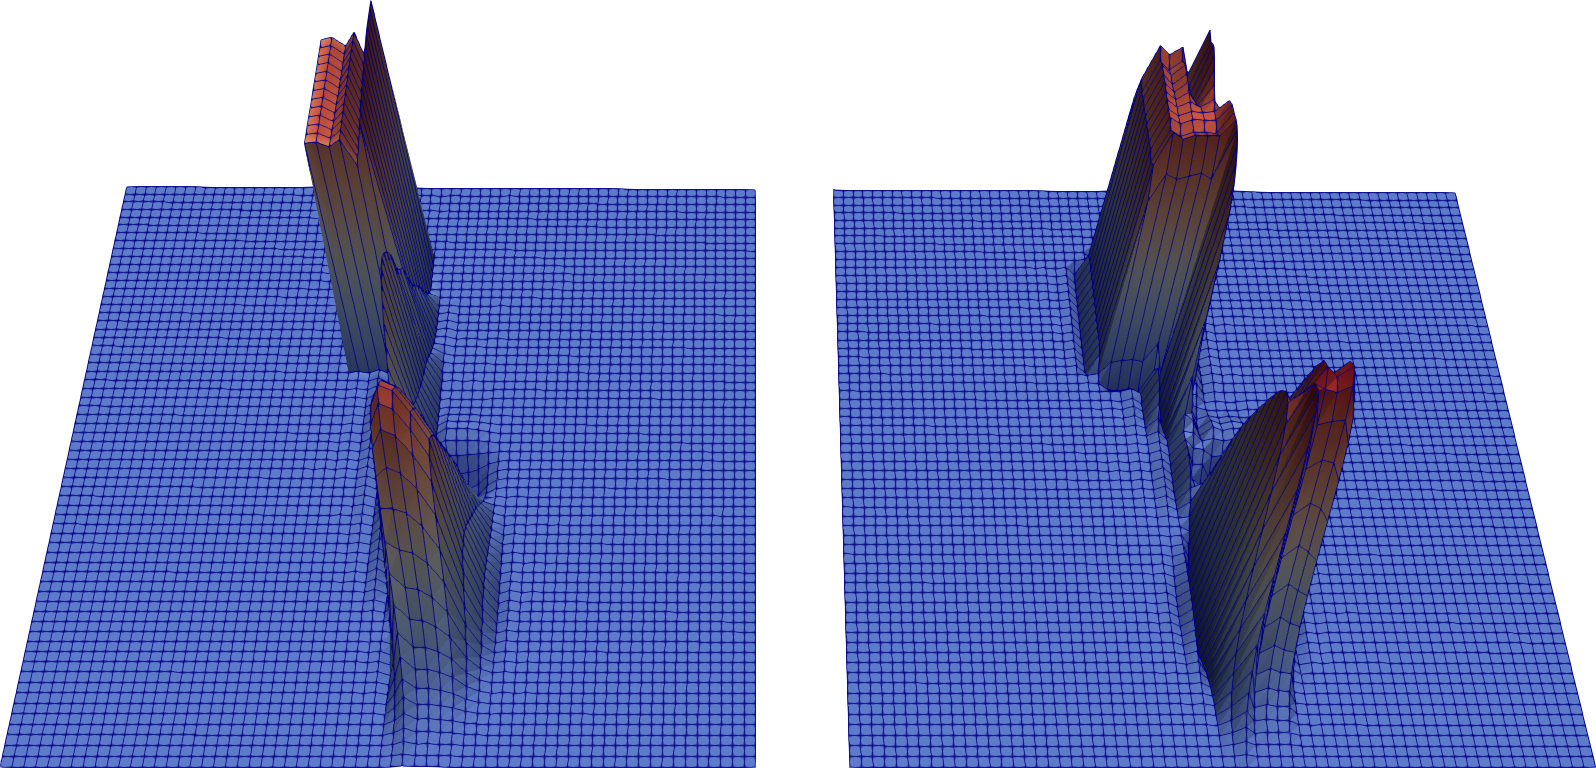
\includegraphics[width=\textwidth]{cookbooks/benchmarks/advection/doc/drop.png}%
  \caption{\it Dropping box benchmark at final time. Left: entropy viscosity. Right: SUPG.}\label{fig:benchmark-drop}
\end{figure}

\begin{figure}[t!]
  \centering
    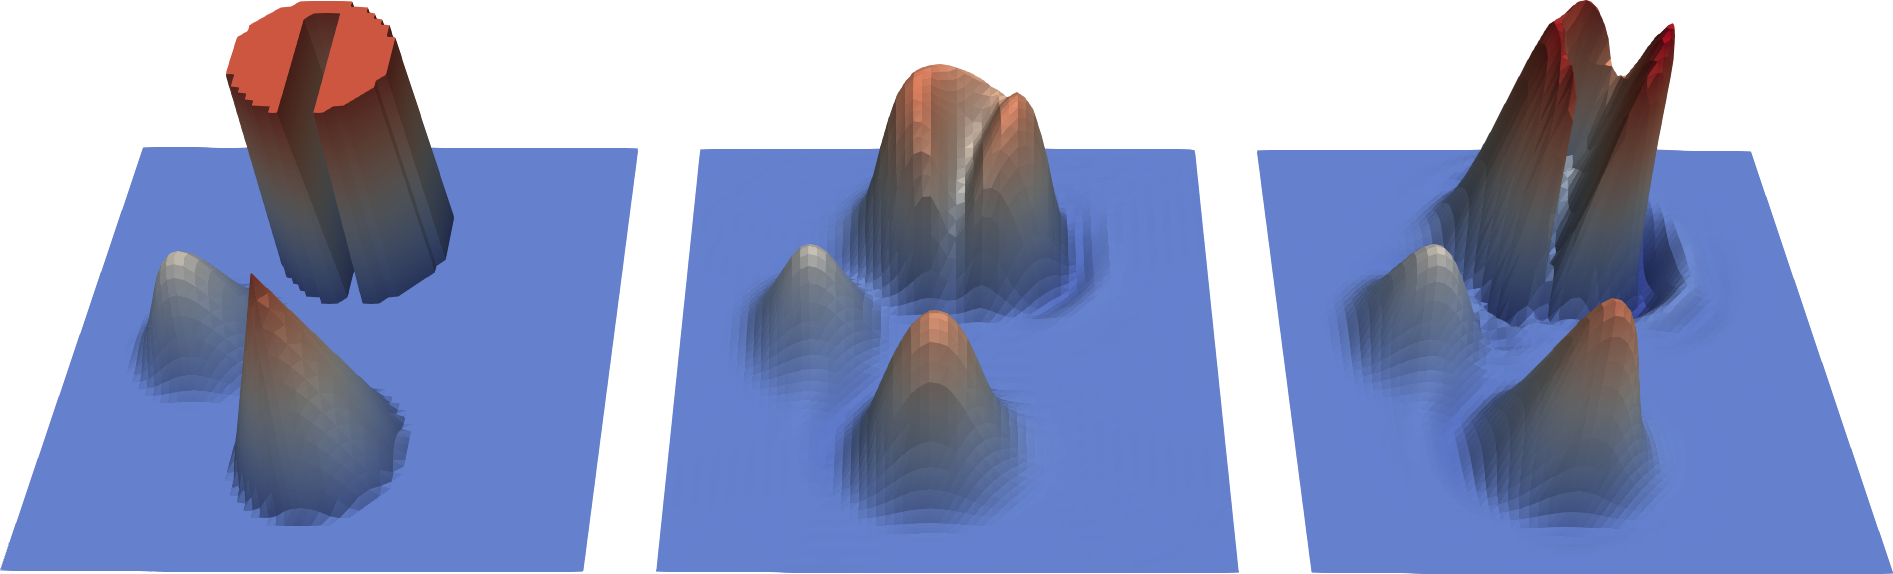
\includegraphics[width=\textwidth]{cookbooks/benchmarks/advection/doc/rotate_shape.png}%
  \caption{\it Rotating shapes benchmark at final time: Left: reference. Middle: Entropy viscosity. Right: SUPG.}\label{fig:benchmark-rotate-shape}
\end{figure}
